\chapter{Background and Related Work \label{chap:background}}

\section{Background}
Manually crafting every animation in the game is unrealistic due to cost and time requirements. Many games have employed various approaches to computer generated animation in order to generate hours of realistic content. No game however has succeded in making the dialogue animation indistinguishable from manually animated cutscenes.

\section{Existing Systems}

There has been a variety of approaches featured in games. Many of them ended up generating dialogue scenes that are higly repetitive, not very realistic and in general not mathing the sentiment and emotion of the speech with movement. The only system that did not seek to find cheap workarounds around the issue and instead embraced the full complexity of the problem is the dialogue sene generator used in The Witcher 3. The system developed by CD Projekt Red made computer generated dialogue sequences in many cases barely distinguishable from those made by an artist, allowing less important scenes to be left completely untouched by a human animator. ~\cite{pcgamerwitcher}


The tool created by CD Projekt Red takes information on initial state of involved characters (position, stance, emotions, etc.) and audio recording of the dialogue lines. The tool chooses matching premade animated clips and outputs a fully editable animated scene of characters conversing with one another. The tool uses audio recordings to aid the animated clips (analyzing the audio waves may help decide when characters accent or underline some information). This tool is the current state-of-the-art and has produced the best effects in terms of amount of work to quality of animation ration. However, there are some serious drawbacks to this project. It still requires a fair amount of work as for every scene the initial state must be specified manually. Moveover, the system requires audio to be recorded first. Moreover, the tool is not released to be used commercially outside CD Projekt. ~\cite{gdcwitcher}


The tool I propose would hardly be able to compete with that of CD Projekt Red, however it would have some significant advantages. It would make generating the scenes even faster (requiring less manual work and preparation) and would in general be more appealing to small developers and people who are not animation experts.

\section{Related Work}
The main focus of this project is the usage of NLP for generating animated sequences. While this project puts particular emphasis on generating scenes of dialogue, there exist a multitude of projects that explores the usage of NLP in animation in a variety of ways.

A very early research (1991) explores usage of NLP for creating animations that would help engineers demonstrate tasks in an easy and safe way (demonstrating tasks personally might be unsafe, reading manuals might be insufficient to understand the task in full)~\cite{animosha}. The system would take as input a set of natural language \textit{directives} or \textit{commands} (e.g. \textit{move cup to table}). The system would interpret such an instruction into a series of steps (tasks) that are carried out in a given order. Based upon that sequence an animation would be generated.

The project hovewer seems to have a few significant problems. Most importantly, the end results was not editable. In my research I believe that the end results will not be immediately satisfactory without any manual improvements and I believe that the outputted scenes should be fully editable. The other issue with this project is that the end result is not realistic or immersive (this was not a priority of that research, but is important for me). The animations were automatically generated in full, which I do not believe to be a viable approach for my project. To improve realism of the scenes, the animation should be created using motion capture clips.

A lot more research has been done in this area with certain degree of success. Another interesting paper explores a topic more similar to the focus of this report. ~\url{Generating Animation from Natural Language Texts and Framework of Motion Database} proposes using a database of pre-recorder motion data instead of filly generating the movements~\cite{animmc}. The paper argues that motion synthesis requires too much manual setup (which a normal user might find too hard). The paper also proposes an architecture of a database -  a way to store motion capture clips and their associated metadata. The system described in this paper is however essentially different from what I propose in this report, as the described report focuses on action-driven animation, while my tool would focus on dialogue-driven animation.

While many other reasearch focused on animation in general, some reasearch focused on usage on NLP generated animation for use in games specifically. It aimed to create a parser that would transform natural language text to a set of instructions for the animation layer. The end goal was realtime character control by natural language commands. The animations were not intended to increase realism, but rather to accomplish goals in a strategic manner. The research was generally succesful proving the potential usefulness of NLP in game development. ~\cite{animpaper3}

So far, the main focus of similar research has been generating animated scenes from text with focus on actions, often by employing motion synthesis. There exists no record of using  sentiment analysis to create animated dialogue scenes.


% ----------------------------------------------- %


\section{Emotion Analysis}

The task of emotion analysis is a subset of natural language processing. The task of analysing natural language text in search of subjective information such as sentiment or emotion is known as sentiment analysis.

\subsection{Sentiment Analysis}
Sentiment Analysis can be broadly defined as a computational approach for discovering opinions and attitudes expressed in text by opinion holders. In its most basic form it focuses on binary classification of the sentiment of the opinion holder (positive or negative) ~\cite{sentimentanal1}, but can be extended to mine for more complicated opinions such as emotions or detecting sarcasm. One of the popular uses of sentiment analysis is predicting stock market behaviour, as well as getting immediate feedback on products, political campaigns, decisions by monitoring social media ~\cite{sentimentanal2}.

Approach to sentiment analysis might differ depending whether focus is on document-level analysis or sentence level analysis - where document-level analysis assumes the entire document to have one clear area of focus, while sentence level analysis analyzes each sentence individually. Apart from those, there are more types of sentiment analysis such as aspect-based analysis (which is use when the document or sentence does not focus on a single entity), or comparative analysis (when direct opinion is not desired, but it is needed to contrast opninions with each other)~\cite{sentimentanal2}. For the purposes of this project, it seems that the sentence-leve approach is the most suitable, as dialogues comprise of mostly single-sentence lines (rarely more than three sentences per line) and emotional payload may change as the dialogue progresses.

Traditionally sentiment analysis is performed by various classification mathods (usually supervised learning). Naive Bayes classifier and support vector machines were proven to yield pretty acurrate results (over 80\% accuracy in general) ~\cite{sentimentanal1}. The major constrait of those methods is that their quality is tightly linked with the quality of the lexicon used and size and quality of training datasets.

One state-of-the-art solution to emotion analysis problem has recently became publicly available. Created by IBM, Watson Tone Analyzer is a tool capable of accurate emotion labeling (fear, joy, anger, etc.) as well as tone labeling (analytical, confident, tantative, etc.). The system is based on the \textit{Big Five personality traits} model ~\cite{watson}. Thanks to this approach, Watson is capable of much more detailed analysis of natural language than most other tools.


\subsection{Emotions}
To fully understand how to approach the problem of animation generation from emotional natural language it is important to look at how can emotions be understood and represented in computational terms. Emotions are complex and subjective in nature, so it is important t deconstruct emotions into something that can be worked with. A traditional approach to this problem is using the six basic emotion model. Specified by Paul Ekman and Wallace V. Friesen, who by studying nativa papua-new guinean tribes have discovered six universally recognized and understood emotions: ~\cite{basicemo}
\begin{itemize}
\item Joy
\item Anger
\item Surprise
\item Disgust
\item Fear
\item Sadness
\end{itemize}

Although various research proposes changes to the six basic emotions model (such as reducing it to just four basic emotions ~\cite{fouremo}), this model is widely accepted and used in literature and software (such as IBM Watson tone analyzer, or various lexicons such as the NRC Word-Emotion Association Lexicon \footnote{\url{http://www.saifmohammad.com/WebPages/NRC-Emotion-Lexicon.htm}}.

Psychologists theorize that the basic emotions can be used as building blocks to achieve more complex emotions. The specific emotion can be described as a mixture of basic emotions and their intensities. Robert Plutchik, a supporter of that theory, has represented emotions on a wheel-like diagram (~\ref{fig:wheel}) that depicts how two basic emotions combine to create a more complex emotion ~\cite{basicemo}.

\begin{figure}[H]
\centerline{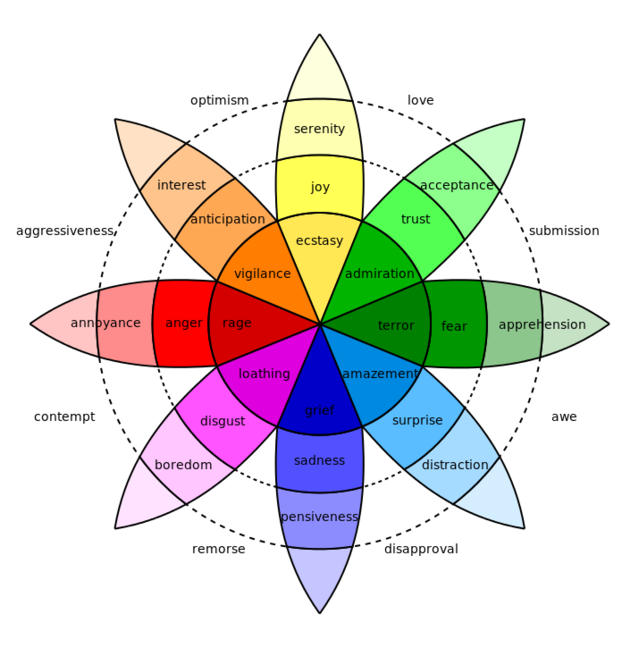
\includegraphics[width = 30em]{img/wheel.png}}
\caption{Plutchik's wheel}\label{fig:wheel}
\end{figure}

It seems that it is enough to extract the very basic emotions from the text, as more complex emotions can be understood as combinations of those basic ones.


\section{Animation Software}
\label{sec:animchoice}

The output scene must be created in some software able to play and use the scene. Developing a tool for this would be too time consuming - such software is not a small undertaking and with the time constraints this would result in a very rudimentary framework that would be very limiting. Therefore a choice must be made between existing frameworks.

The animation software must satisfy the following requirements:
\begin{itemize}
\item Flexibility and editability - As the scenes created by the generator will not be perfect, the software must provide powerful animation editing features.
\item Exporting - It is desirable for the animation to be able to be exported into variety of different formats that can be used by other frameworks useful within game development.
\item Availability - As the proposed tool is developed with small developers in mind, it is most desirable for the tool to be available without any unnecessary fees or licensing. The proposed tool shoul also provide help for people unfamiliar with animating, who would be unwilling to pay additional fees for something they are not familiar with.
\item Familiarity - Although most animation software is based on similar concepts, due to time constraints my previous experience with the software is also important.
\end{itemize}


\subsection{Maya}
Maya is a 3D computer animation software developed by Autodesk. It supports modeling, rendering, simulation, texturing, and animation. This software is an industry standard and has been used for such projects as the Halo franchise. It supports all the animation editing and exporting features needed for this project, however it comes with a pretty harsh pricetag of \$180 per month \footnote{\url{https://www.autodesk.com/products/maya/subscribe}}; a price which would make the potential reach of the proposed tool much smaller. Moreover, although I am familiar with animation concepts, I am not familiar with Maya.


\subsection{Blender}
Blender is an open source animation software. Similarly to Maya, it supports modeling, rendering, simulation, texturing and animation. Due to its open source nature the software may be less usable or stable at times however it is still very powerful and recognized within the industry. Blender's rendering engines are not as sophisticated as those of Maya. It supports exporting the animations to Collada, Alembic, 3D Studio, FBX, Motion Capture (.bvh), Wavefront, X3D and Stl file formats. This means that the final animation could be exported and used by pretty much any other tool. Blender is completely free to use and available to anyone. I am familiar with the tool


\subsection{Unreal Engine}

Unreal Engine is by far the most popular and most powerful publicly accessible game engine. Since the proposed tool would find most use in games it would make sense to create the scenes directly in a game engine. This approach however has some disadvantages - animation editing features in game engines are much more limited than those of a software dedicated to creating animation. Moreover, any game engine will not support the same exporting features (however, since the animation would already be in the engine, the need for exporting is arguable). Unreal engine is free to use, however Epic Games will seize a portion of income generated by a product developed with Unreal Engine. \footnote{\url{https://www.unrealengine.com/en-US/faq}}

\subsection{Unity 3D}

Unity 3D is the most popular freely available engine after Unreal. It suffers from the same drawbacks regarding animation editing features and is in general less stable and sophisticated. The only reason why Unity would be more suitable than Unreal for this project is my familiarity with the Unity 3D framework.


\subsection{Final Choice}

Upon taking a closer look on the available software, I conclude that Blender is the most suitable tool for the task as it satisfies the requirements best. It provides all the necessary editing exporting and editing features, is free and easily available and I already have experience with using it.



\section{Motion Database}

The dialogue scenes in this project are going to be assembled from existing short motion capture clips. While a potential user of the tool proposed by this paper (a game studio) would most likely possess resources to create their own motion capture clips and be in posession of legacy motion capture data recorded for past projects, I must resort to use other resources. There exists a multitude of motion capture data freely available online\footnote{\url{http://jeroenvanboxtel.com/MocapDatabases.html}}. Among them, the most famous is the Carneigie Mellon University's CMU Graphics Motion Capture Database\footnote{\url{http://mocap.cs.cmu.edu/}}. It contains thousands of recordings of people walking, dancing, running, performing everyday activities, playing sports and performing gestures.

Only a small portion of that database would be useful to this project. There is however another database that focuses on matters more aligned with this project - the Emotional Body Motion Database \footnote{\url{http://ebmdb.tuebingen.mpg.de/index.php}}. The database was created by the Max Planck Institute for Biological Cybernetics and features solely recordings of people performing gestures associated with some emotion. The recordings feature all the basic emotions listed earlier as well as other emotions such as pride, relief, shame and more. There are three main types of motion capture recordings in this database:
\begin{itemize}
\item Narration - Actors were recorded while reading a story - their gestures were captured while narrating a part of the story that emphasizes some emotion.
\item Nonverbal - Actors were recorded performing a gesture associated with some emotion in a nonverbal setting.
\item Sentence - Actor were recorder while performing gestures when talking.
\end{itemize}
The database contains over 1400 clips, each labeled with what emotion it is supposed to represent, and what emotion would an observer assoiate the recording with ~\cite{planck1}~\cite{planck2}. An example entry in the EBMD can be seen in ~\ref{fig:ebmd1}.

\begin{figure}[H]
\centerline{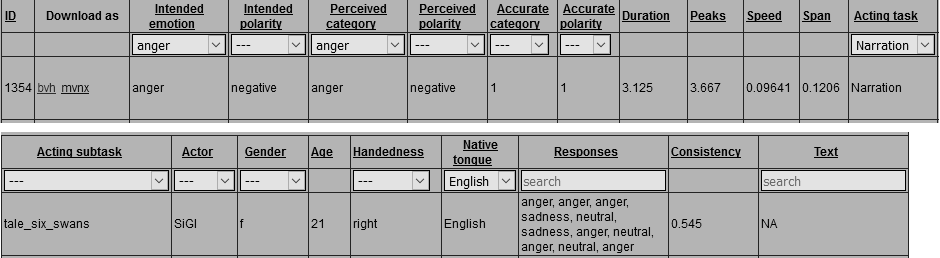
\includegraphics[width = 30em]{img/emo1.png}}
\caption{An example emdb entry}\label{fig:ebmd1}
\end{figure}


\section{Uncanny Valley}

When dealing with animation, modelling, sculpting, etc. it is important to remember about the phenomenon of the uncanny valley. Not taking this phenomenon into account might cause unexpected negative results.

\subsection{What is the uncanny valley}

The uncanny valley is a phenomen regards aesthetics. It states that when a humanoid object (a character model, a robot) behaves in a more realistic, human-like fashion, it might not be necessairly perceived as more human-like. The \textit{valley} suggests that there exists a certain \textit{dip} in human observer's affinity for a human replica ~\cite{uncanny1}.

The concept was first identified byrobotics professor Masahiro Mori in 1970. In his essay on the uncanny valley he explains the relationship between a humanoid object's human likeness and observer's affinity towards the object. He has noted, that as the object becomes more human like, the observer's affinity increases. However, when the human likeness of the object reaches certain point, the human affinity for it decreases drastically. Then again, when the human likeness becomes very high, the affinity drastically rises again. The observers might perceive humanoid objects that are not quite human like as funny, cute, in need of repair, etc. The obsever perceive very human like objects are almost indistinguishable from reality - and while they may not be perfect, there is nothing alarming about them. However, the observers have described \textit{fairly} human like humanoid replicas as \textit{creepy} or \textit{eerie} ~\cite{uncanny1}~\cite{uncanny2}.

The concept is easily depicted on a graph. Figure ~\ref{fig:uncanny} draws the relationship between human likeness and observer affinity. According to this representation, when a replica's human likeness reaches about 80\%, observers affinity quickly becomes negative. Figures ~\ref{fig:toyrobot}~\ref{fig:uncannyrobot}~\ref{fig:realrobot} shows an example of this concept, by showing three different robot examples and their relation to the uncanny valley principle. 

\begin{figure}[H]
\centerline{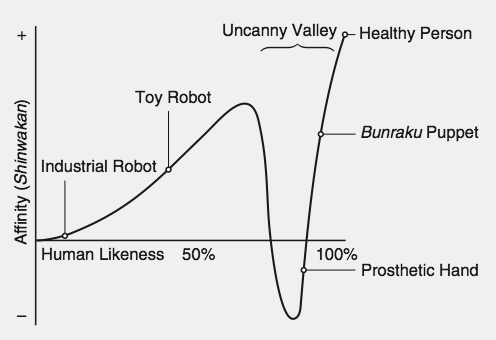
\includegraphics[width = 30em,scale=0.25]{img/uncanny.png}}
\caption{The uncanny valley}\label{fig:uncanny}
\end{figure}

\begin{figure}[H]
\centerline{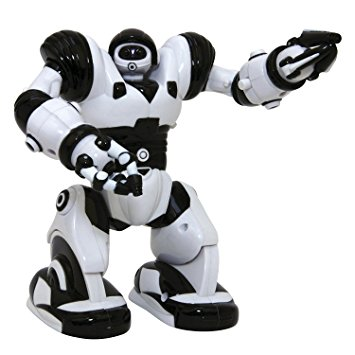
\includegraphics[scale=0.4]{img/toyrobot.jpg}}
\caption{This robot does not fall into the uncanny valley category. It is a humanoid but it is not realistic - it is usually perceived as funny or cute.}\label{fig:toyrobot}
\end{figure}

\begin{figure}[H]
\centerline{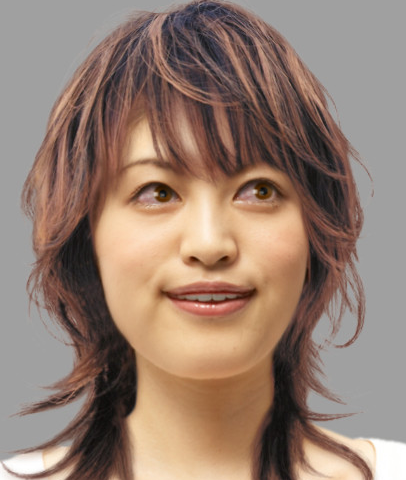
\includegraphics[scale=0.4]{img/uncannyrobot.png}}
\caption{A robot that falls into the uncanny valley category - It is realistic enough to be human-like, but it is not human-like enough to be perceived positively and described as realistic. It provokes a feeling of eerieness or being alarmed in the observers.}\label{fig:uncannyrobot}
\end{figure}

\begin{figure}[H]
\centerline{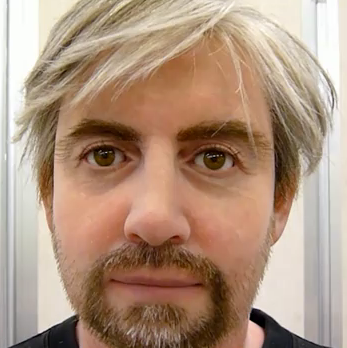
\includegraphics[scale=0.45]{img/realrobot.png}}
\caption{This robot does not fall into the uncanny valley as it is realistic enough to feel familiar and normal.}\label{fig:realrobot}
\end{figure}

\subsection{Why uncanny valley matters in games and animation}

Since animation and modelling deals with humanoid objects, the uncanny valley principle applies to it as well. Many game studios h will prefer to use comic-like graphics and other solutions in order to purposefully make the game less realistic. Oftentimes a less realistic game will be received better than a game that is quite realistic but not exactly so. Characters that fall into the uncanny valley category are often no longer perceived as humans, they are not realatable and laughable ~\cite{uncannygames}.

This problem is exactly what caused the specacular failure of Mass Effect Andromeda. BioWare's  process of creating large amounts of dialogue animation has produced animations which are quite realistic but do not feel human. The players quickly lost interest in the characters, as serious scenes behaved in a fashion that was out of place, unpredictable, and did not highlight emotions they were trying to convey through speech. The case study of this game shows not only why a good system of generating animation is important, but also that a generation system that is generally realistic might be too little and too much at the same time ~\cite{uncannyandromeda}.

This project is also subject to uncanny valley. This principle might cause a set of pretty decent computer generated animations to be perceived very negatively by the audience. I will evaluate on that in section ~\ref{sec:riskanal}.






